\section{Klassifikation}
Für die Beurteilung der Klassifikation, die in Kapitel \ref{kap:klassifikation} beschrieben wurde, wird eine
Wahrheitsmatrix\cite{wiki:confusion_matrix} (engl. \emph{confusion matrix}) verwendet.
Daraus können Metriken berechnet werden, welche eine Aussage über die Qualität der Klassifikation erlauben.

In Tabelle \ref{tab:klassifikation_resultate_confusion_matrix} ist die Wahrheitsmatrix der Testdaten
für die Klassifikation aufgeführt. Es wurden 32 Testbilder erstellt, wobei jeweils alle farbigen und einige rote Kugeln
auf jedem Bild abgebildet sind. Dies führt dazu, dass es mehr Testdaten für die roten Kugeln gibt als für die anderen farbigen Kugeln.
In den Testbildern sind keine Kugeln mit der Klasse \emph{unknown} vorhanden.

Aus der Wahrheitsmatrix ist ersichtlich, dass braune und rote Kugeln teilweise verwechselt werden.
Dies ist auf die ungleichmässige Ausleichtung des Billardtisches zurückzuführen, wodurch eine genaue Unterscheidung
der roten und braunen Kugeln schwierig ist.
In Abbildung \ref{fig:classification_results_failed_examples} sind einige dieser falsch klassifizierten Kugeln abgebildet.
Die restlichen Kugelfarben werden sehr gut klassifiziert. Keiner der Kugeln wurde die Klasse \emph{unknown} zugewiesen.
Die Vertrauenswahrscheinlichkeit\cite{wiki:beurteilung_binärer_klassifikator} (engl. accuracy) beträgt 96\%.

\begin{figure}[h!]
        \centering
        \begin{subfigure}[t]{0.2\textwidth}
                \centering
                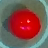
\includegraphics[width=1.0\linewidth]{../common/04_results/resources/classification/failed_classification_BROWN_RED_7_original.png}
                \caption{Rote Kugel klassifiziert als braune Kugel}
                \label{fig:classification_results_failed_classification_BROWN_RED_7_original}
        \end{subfigure}
        \hfill
        \begin{subfigure}[t]{0.2\textwidth}
                \raggedright
                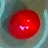
\includegraphics[width=1.0\linewidth]{../common/04_results/resources/classification/failed_classification_BROWN_RED_12_original.png}
                \caption{Rote Kugel klassifiziert als braune Kugel}
                \label{fig:classification_results_failed_classification_BROWN_RED_12_original}
        \end{subfigure}
        \hfill
        \begin{subfigure}[t]{0.2\textwidth}
                \raggedright
                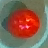
\includegraphics[width=1.0\linewidth]{../common/04_results/resources/classification/failed_classification_RED_BROWN_3_original.png}
                \caption{Braune Kugel klassifiziert als rote Kugel}
                \label{fig:classification_results_failed_classification_RED_BROWN_3_original}
        \end{subfigure}
        \hfill
        \begin{subfigure}[t]{0.2\textwidth}
                \raggedright
                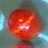
\includegraphics[width=1.0\linewidth]{../common/04_results/resources/classification/failed_classification_RED_BROWN_6_original.png}
                \caption{Braune Kugel klassifiziert als rote Kugel}
                \label{fig:classification_results_failed_classification_RED_BROWN_6_original}
        \end{subfigure}
        \hfill
        \begin{subfigure}[t]{0.2\textwidth}
                \centering
                
\includegraphics[width=1.0\linewidth]{../common/04_results/resources/classification/failed_classification_BROWN_RED_7_roi.png}
                \caption{Bildausschnitt für Abbildung \ref{fig:classification_results_failed_classification_BROWN_RED_7_original}}
                \label{fig:classification_results_failed_classification_BROWN_RED_7_roi}
        \end{subfigure}
        \hfill
        \begin{subfigure}[t]{0.2\textwidth}
                \raggedright
                
\includegraphics[width=1.0\linewidth]{../common/04_results/resources/classification/failed_classification_BROWN_RED_12_roi.png}
                \caption{Bildausschnitt für Abbildung \ref{fig:classification_results_failed_classification_BROWN_RED_12_original}}
                \label{fig:classification_results_failed_classification_BROWN_RED_12_roi}
        \end{subfigure}
        \hfill
        \begin{subfigure}[t]{0.2\textwidth}
                \raggedright
                
\includegraphics[width=1.0\linewidth]{../common/04_results/resources/classification/failed_classification_RED_BROWN_3_roi.png}
                \caption{Bildausschnitt für Abbildung \ref{fig:classification_results_failed_classification_RED_BROWN_3_original}}
                \label{fig:classification_results_failed_classification_RED_BROWN_3_roi}
        \end{subfigure}
        \hfill
        \begin{subfigure}[t]{0.2\textwidth}
                \raggedright
                
\includegraphics[width=1.0\linewidth]{../common/04_results/resources/classification/failed_classification_RED_BROWN_6_roi.png}
                \caption{Bildausschnitt für Abbildung \ref{fig:classification_results_failed_classification_RED_BROWN_6_original}}
                \label{fig:classification_results_failed_classification_RED_BROWN_6_roi}
        \end{subfigure}
        \caption{
                Auswahl aus den falsch klassifizierten Kugeln.
                Oben sind die vollständigen Bilder der Kugeln, unten die für die Klassifikation verwendeten Bildausschnitte.
        }
        \label{fig:classification_results_failed_examples}
\end{figure}

% Total accuracy: 0.962054
\begin{table}[ht]
\rowcolors{1}{\seccolor!10}{\seccolor!10} % Rows with 10% of secondary color
\begin{tabular}{ ccccccccccc }
        \rowcolor{\seccolor!50}
        &         & \multicolumn{9}{c}{\textbf{Wahre Farbe}}\\
        &         &   BROWN &    PINK &     RED &   BLACK &  YELLOW &   WHITE &    BLUE &   GREEN & UNKNOWN \\
        & BROWN   &      26 &       0 &      11 &       0 &       0 &       0 &       0 &       0 &       0 \\
        & PINK    &       0 &      32 &       0 &       0 &       0 &       0 &       0 &       0 &       0 \\
        & RED     &       6 &       0 &     213 &       0 &       0 &       0 &       0 &       0 &       0 \\
        & BLACK   &       0 &       0 &       0 &      32 &       0 &       0 &       0 &       0 &       0 \\
        & YELLOW  &       0 &       0 &       0 &       0 &      32 &       0 &       0 &       0 &       0 \\
        & WHITE   &       0 &       0 &       0 &       0 &       0 &      32 &       0 &       0 &       0 \\
        & BLUE    &       0 &       0 &       0 &       0 &       0 &       0 &      32 &       0 &       0 \\
        & GREEN   &       0 &       0 &       0 &       0 &       0 &       0 &       0 &      32 &       0 \\
        \multirow{-10}{*}{\rotatebox{90}{\textbf{Klassifizierte Farbe}}} & UNKNOWN &       0 &       0 &       0 &       0 &       0 &       0 &       0 &       0 &       0
\end{tabular}
\caption{Ergebnisse Klassifikation der Kugelfarben}
\label{tab:klassifikation_resultate_confusion_matrix}
\end{table}
